\documentclass[aspectratio=169,10pt]{beamer}
\usetheme{default}
\usecolortheme{default}
\usepackage{graphicx}
\usepackage{booktabs}
\usepackage{amsmath}
\usepackage[T1]{fontenc}
\setbeamertemplate{navigation symbols}{}
\setbeamerfont{frametitle}{size=\large}
\title[Low-precision CLEAN]{Quantizing the Hogbom CLEAN pipeline to float16/bfloat16\\-- float64 baseline first}
\author{2026 internship -- J. archive, v2 restart}
\date{\today}

\begin{document}

\begin{frame}
\titlepage
\end{frame}

\begin{frame}{Goal and perimeter}
\begin{itemize}
\item Goal: measure the effect of quantizing each stage of the Hogbom CLEAN
  pipeline (visibilities, dirty image, PSF, clean model) to float16/bfloat16,
  against a float64 baseline.
\item Rule for this restart: \textbf{no quantization claim before the f64
  baseline is clean, deterministic, and unit-tested.}
\item Perimeter: MeerKAT 1 h / 4 ch / 1.4 GHz uv-coverage, 1\textdegree{} FOV,
  2520$^2$ images, $\sigma=10^{-4}$ Jy/vis, point + Gaussian sky ladder
  (DR 1$\to$1000), Hogbom. OSKAR-compatible datasets (same layout; canonical
  re-simulation via OSKAR/singularity on a host that has it).
\end{itemize}
\end{frame}

\begin{frame}{Experimental design}
\begin{itemize}
\item uv-coverage harvested from a real OSKAR dataset (725,760 rows $\times$ 4 ch);
  visibilities forward-modelled with ducc0 (exact adjoint gridding) + seeded
  Gaussian noise $\to$ deterministic datasets, reproducible from seed.
\item Sky ladder: S0 = 1 point (DR 1), S1 = 8 points (DR 10),
  S2 = 6 points + 4 gaussians (DR 100), S3 = 4 points + 8 gaussians (DR 1000).
  Realized DR pinned exactly; 3 noise seeds per sky.
\item CLEAN tuning (validated on the legacy archive): Högbom
  $\gamma=0.1$, $pf=10^{-4}$, 10 major cycles; residual re-imaged through the
  visibilities each major cycle.
\item Metrics (all unit-tested, analytic ground truths, 30 tests green):
  cross-correlation of restored images, flux conservation
  $\sum m/\sum t$, residual MAD (Jy/beam), achieved DR = peak/residual-MAD.
\end{itemize}
\end{frame}

\begin{frame}{Pipeline and quantization points}
\begin{center}
visibilities $\xrightarrow{\;q_{vis}\;}$ dirty image $\xrightarrow{\;q_{dirty}\;}$
CLEAN loop $\xrightarrow{\;q_{model}\;}$ model, PSF $\xrightarrow{\;q_{psf}\;}$
\end{center}
\begin{itemize}
\item Quantization = IEEE-754 value rounding (vectorized; f16 with rescale to
  65503 for range), applied per stage; pipeline math stays in f64 on the
  de-scaled values.
\item Self-describing results: every run writes arrays + all parameters +
  metrics (results.npz, params.json, metrics.json).
\end{itemize}
\end{frame}

\section{float64 baseline}

\begin{frame}{Baseline: S0 (1 point source, DR 1) — metrics}
\begin{tabular}{lrrrrr}
\toprule
dataset & seed & cc & flux & res. MAD & ach. DR \\
\midrule
S0\_point1\_n103 & 103 & 1.00000 & 1.00000 & 7.21e-08 & 1.39e+07 \\
\bottomrule
\end{tabular}
\end{frame}

\begin{frame}{Baseline: S0 — images}
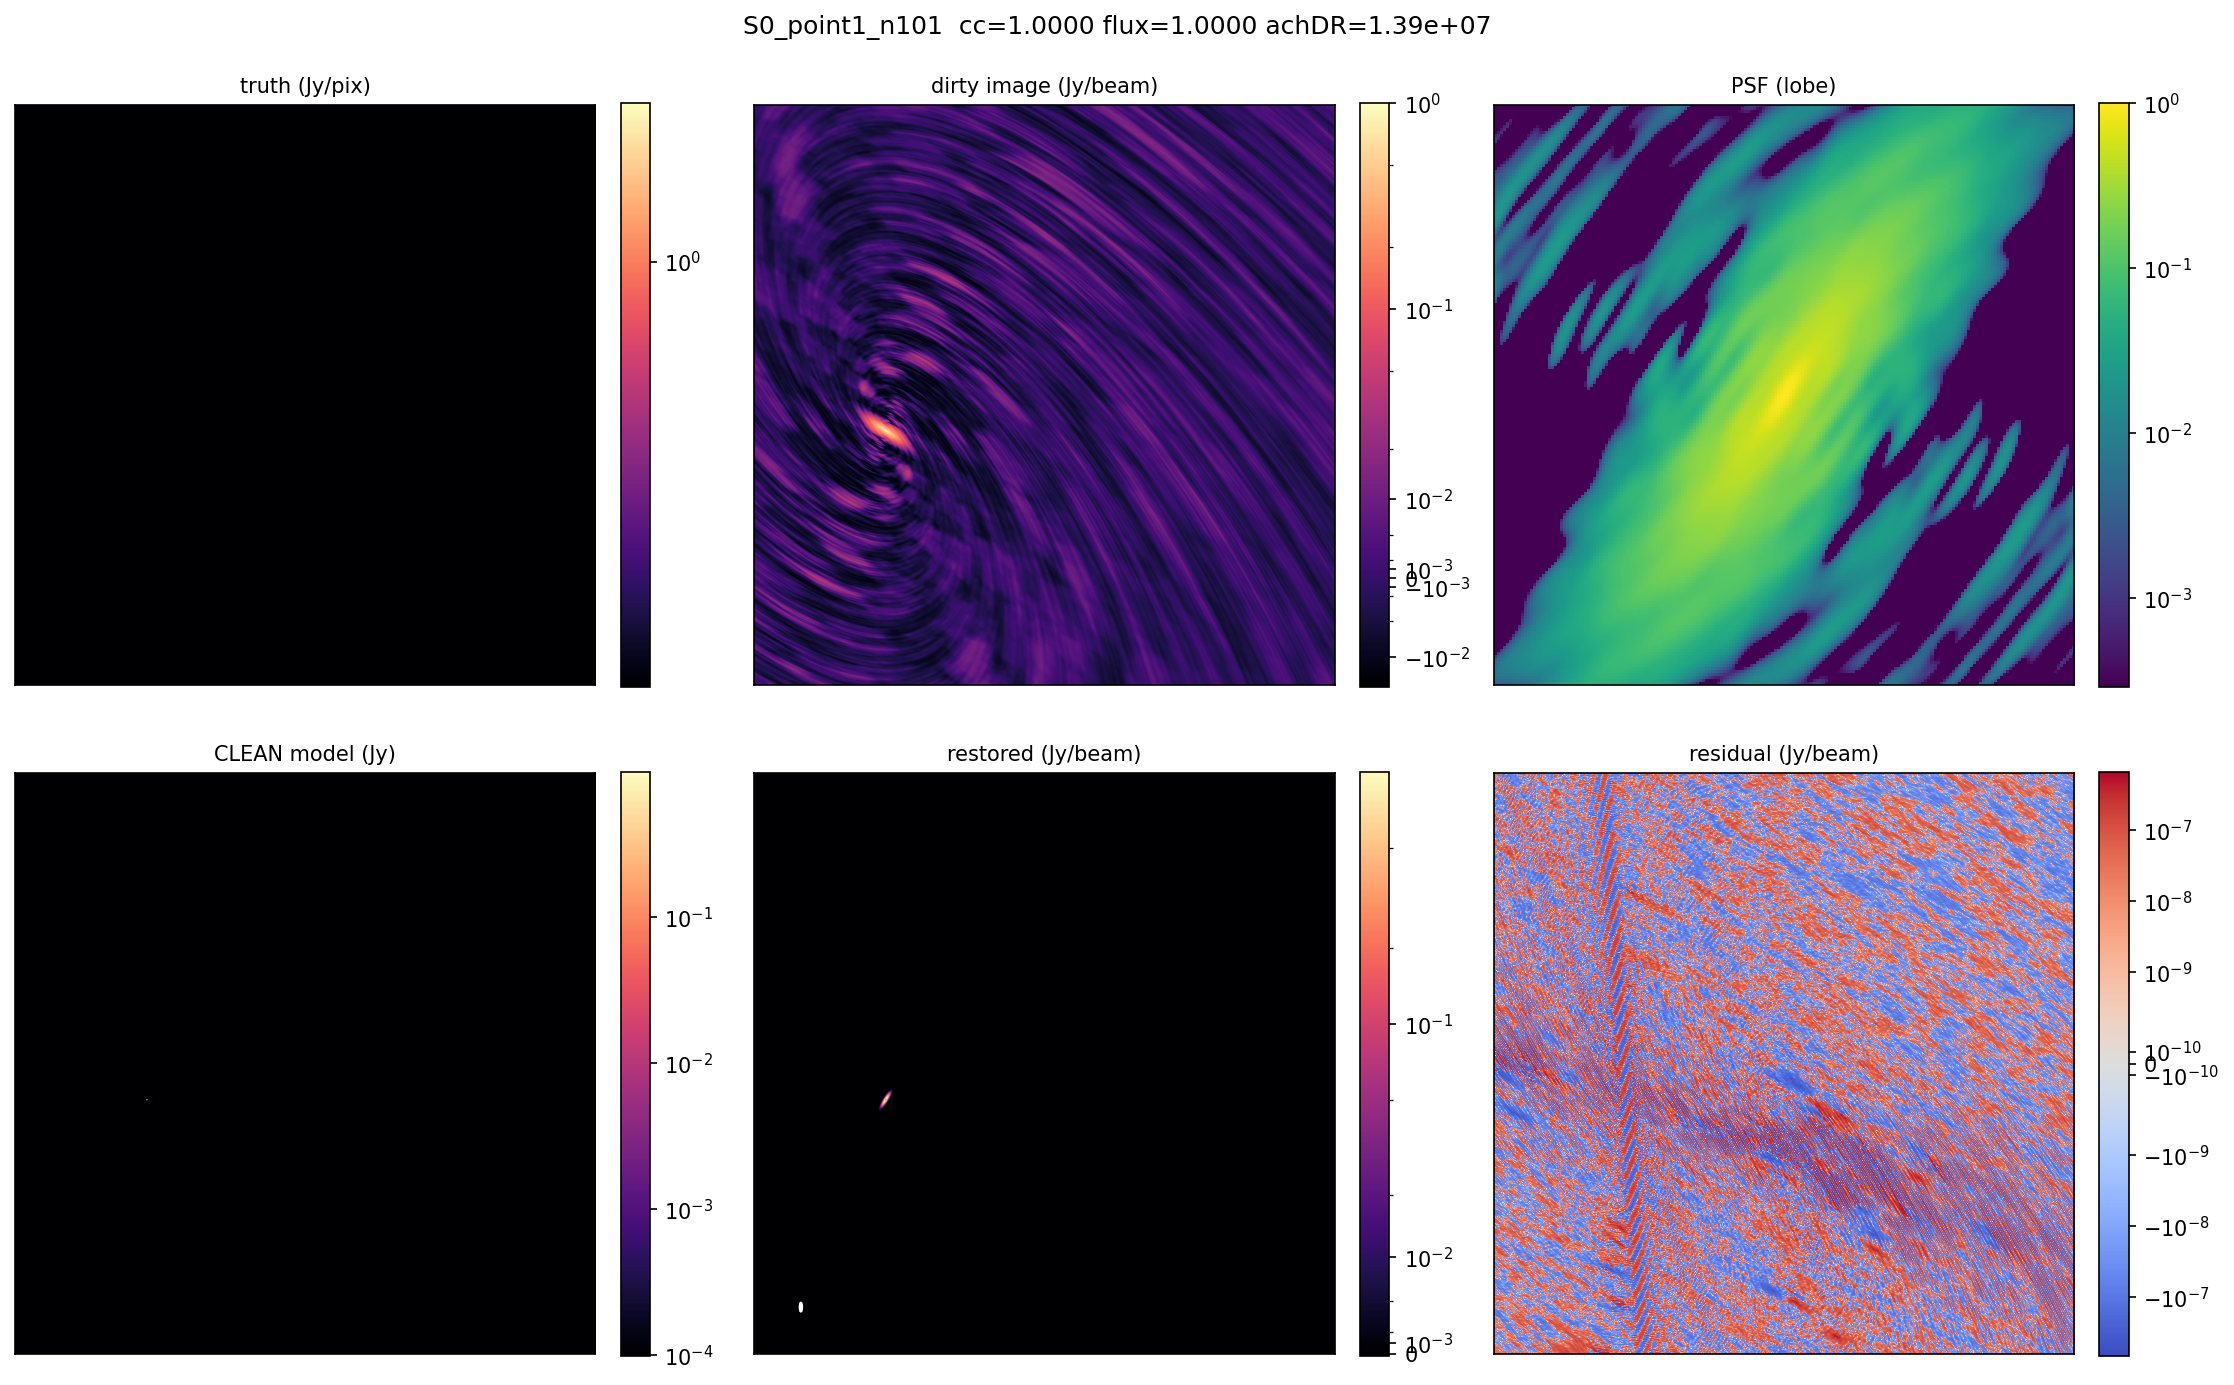
\includegraphics[width=\textwidth]{../analysis/figures/panel_S0_point1_n101.png}
\end{frame}

\begin{frame}{Baseline: S1 (8 points, DR 10) — images}
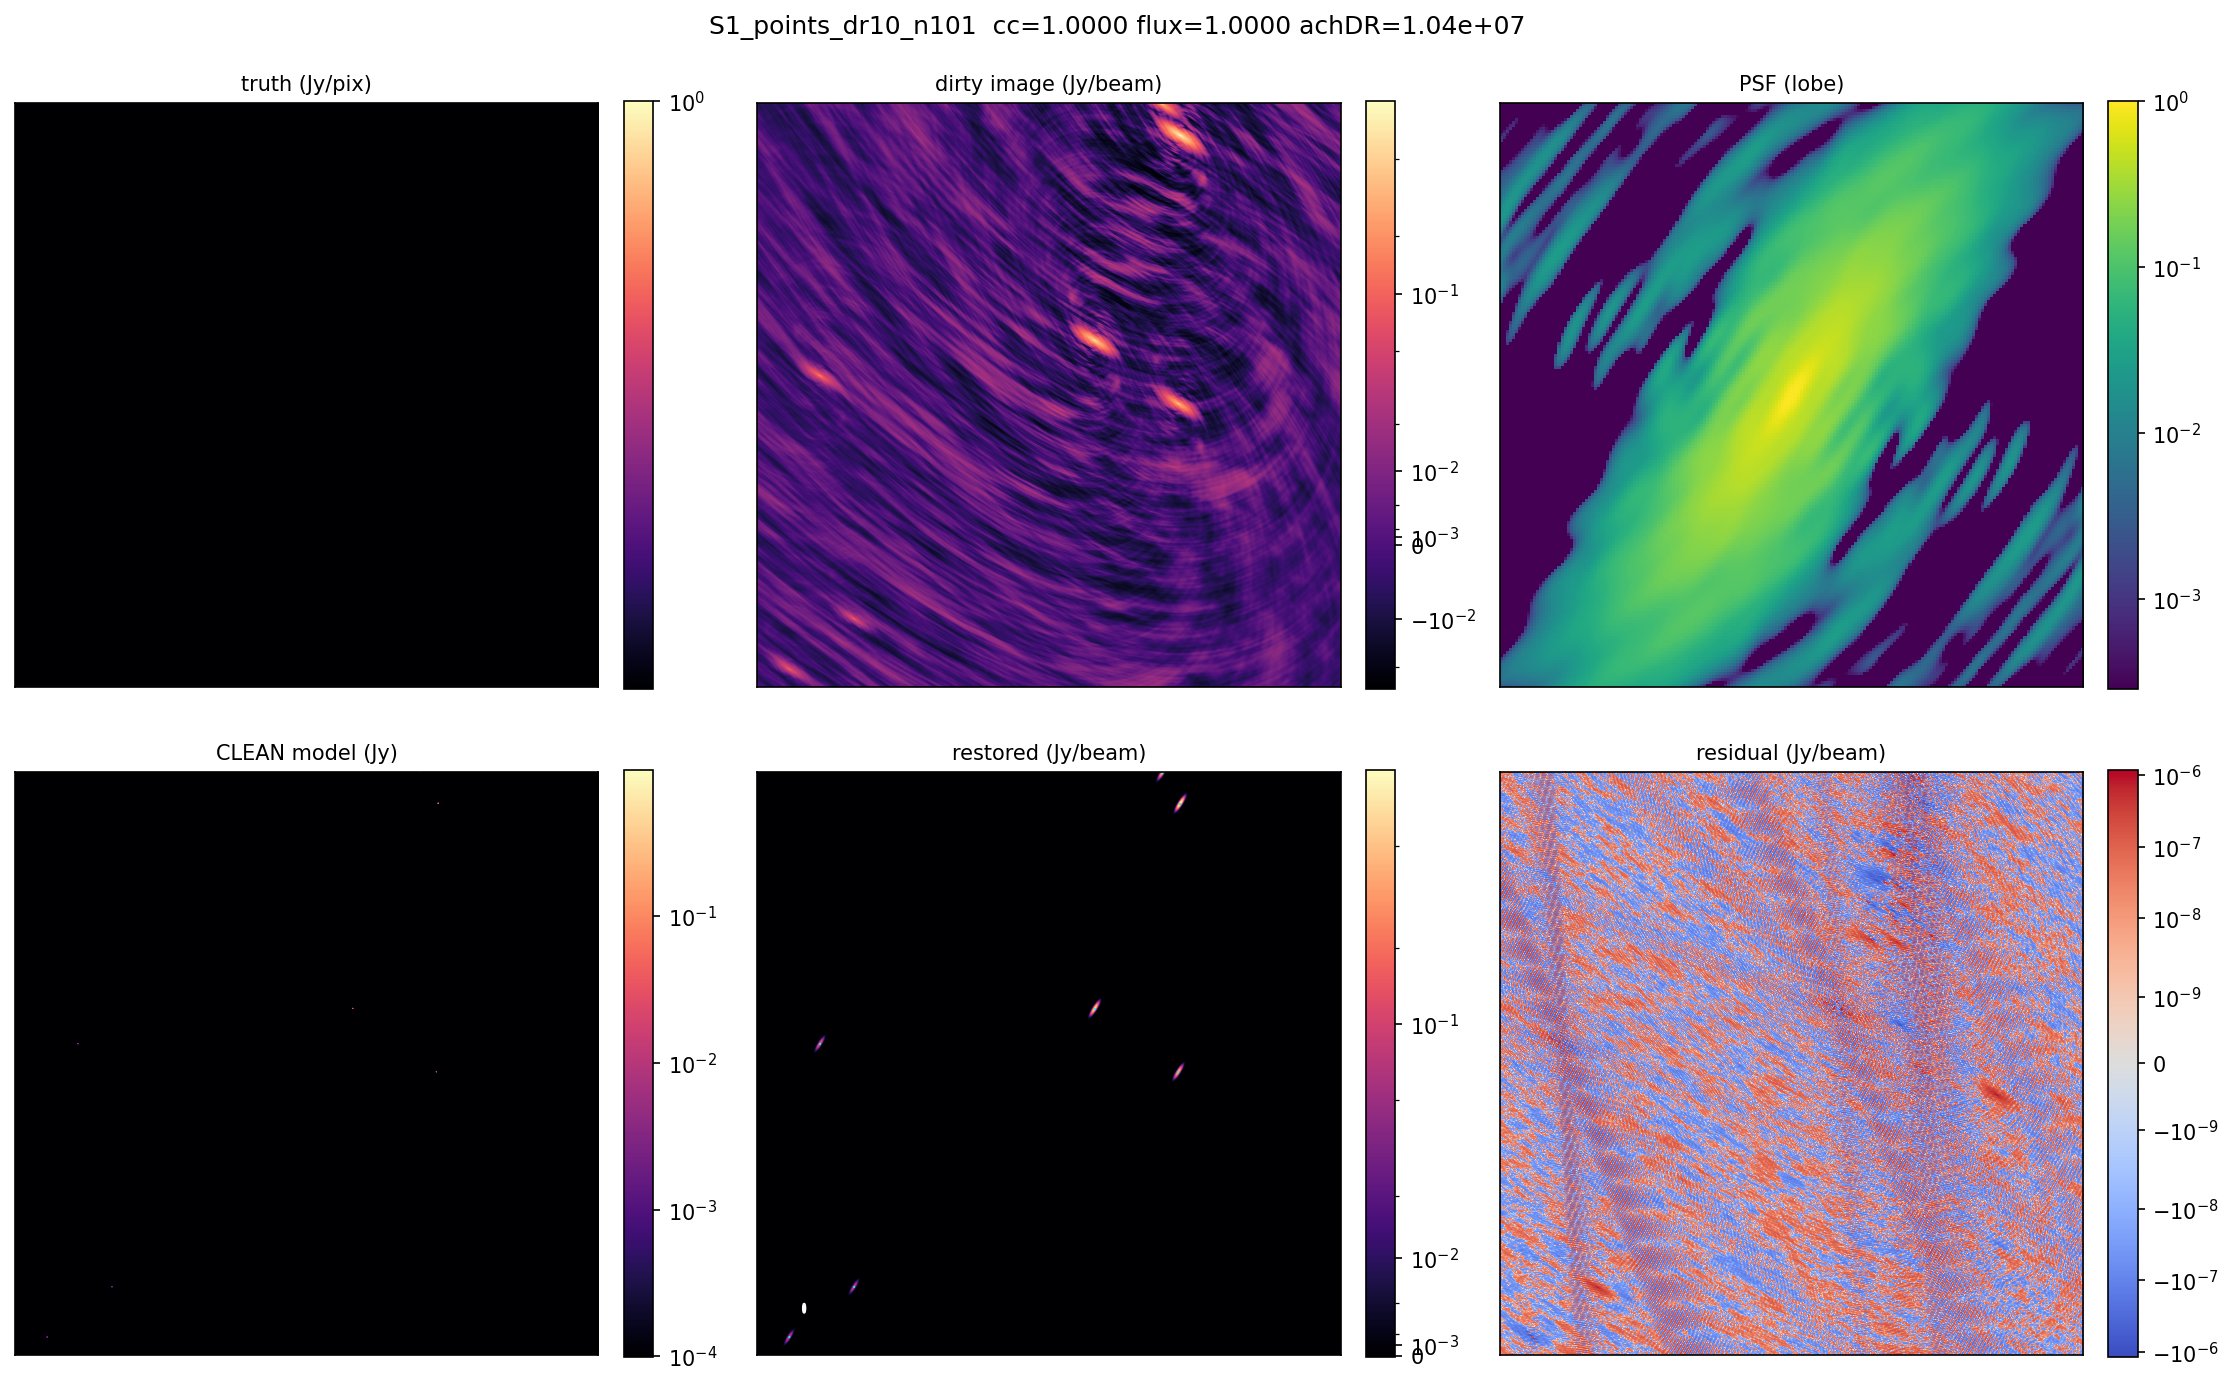
\includegraphics[width=\textwidth]{../analysis/figures/panel_S1_points_dr10_n101.png}
\end{frame}

\begin{frame}{Baseline: S2 (points + gaussians, DR 100) — images}
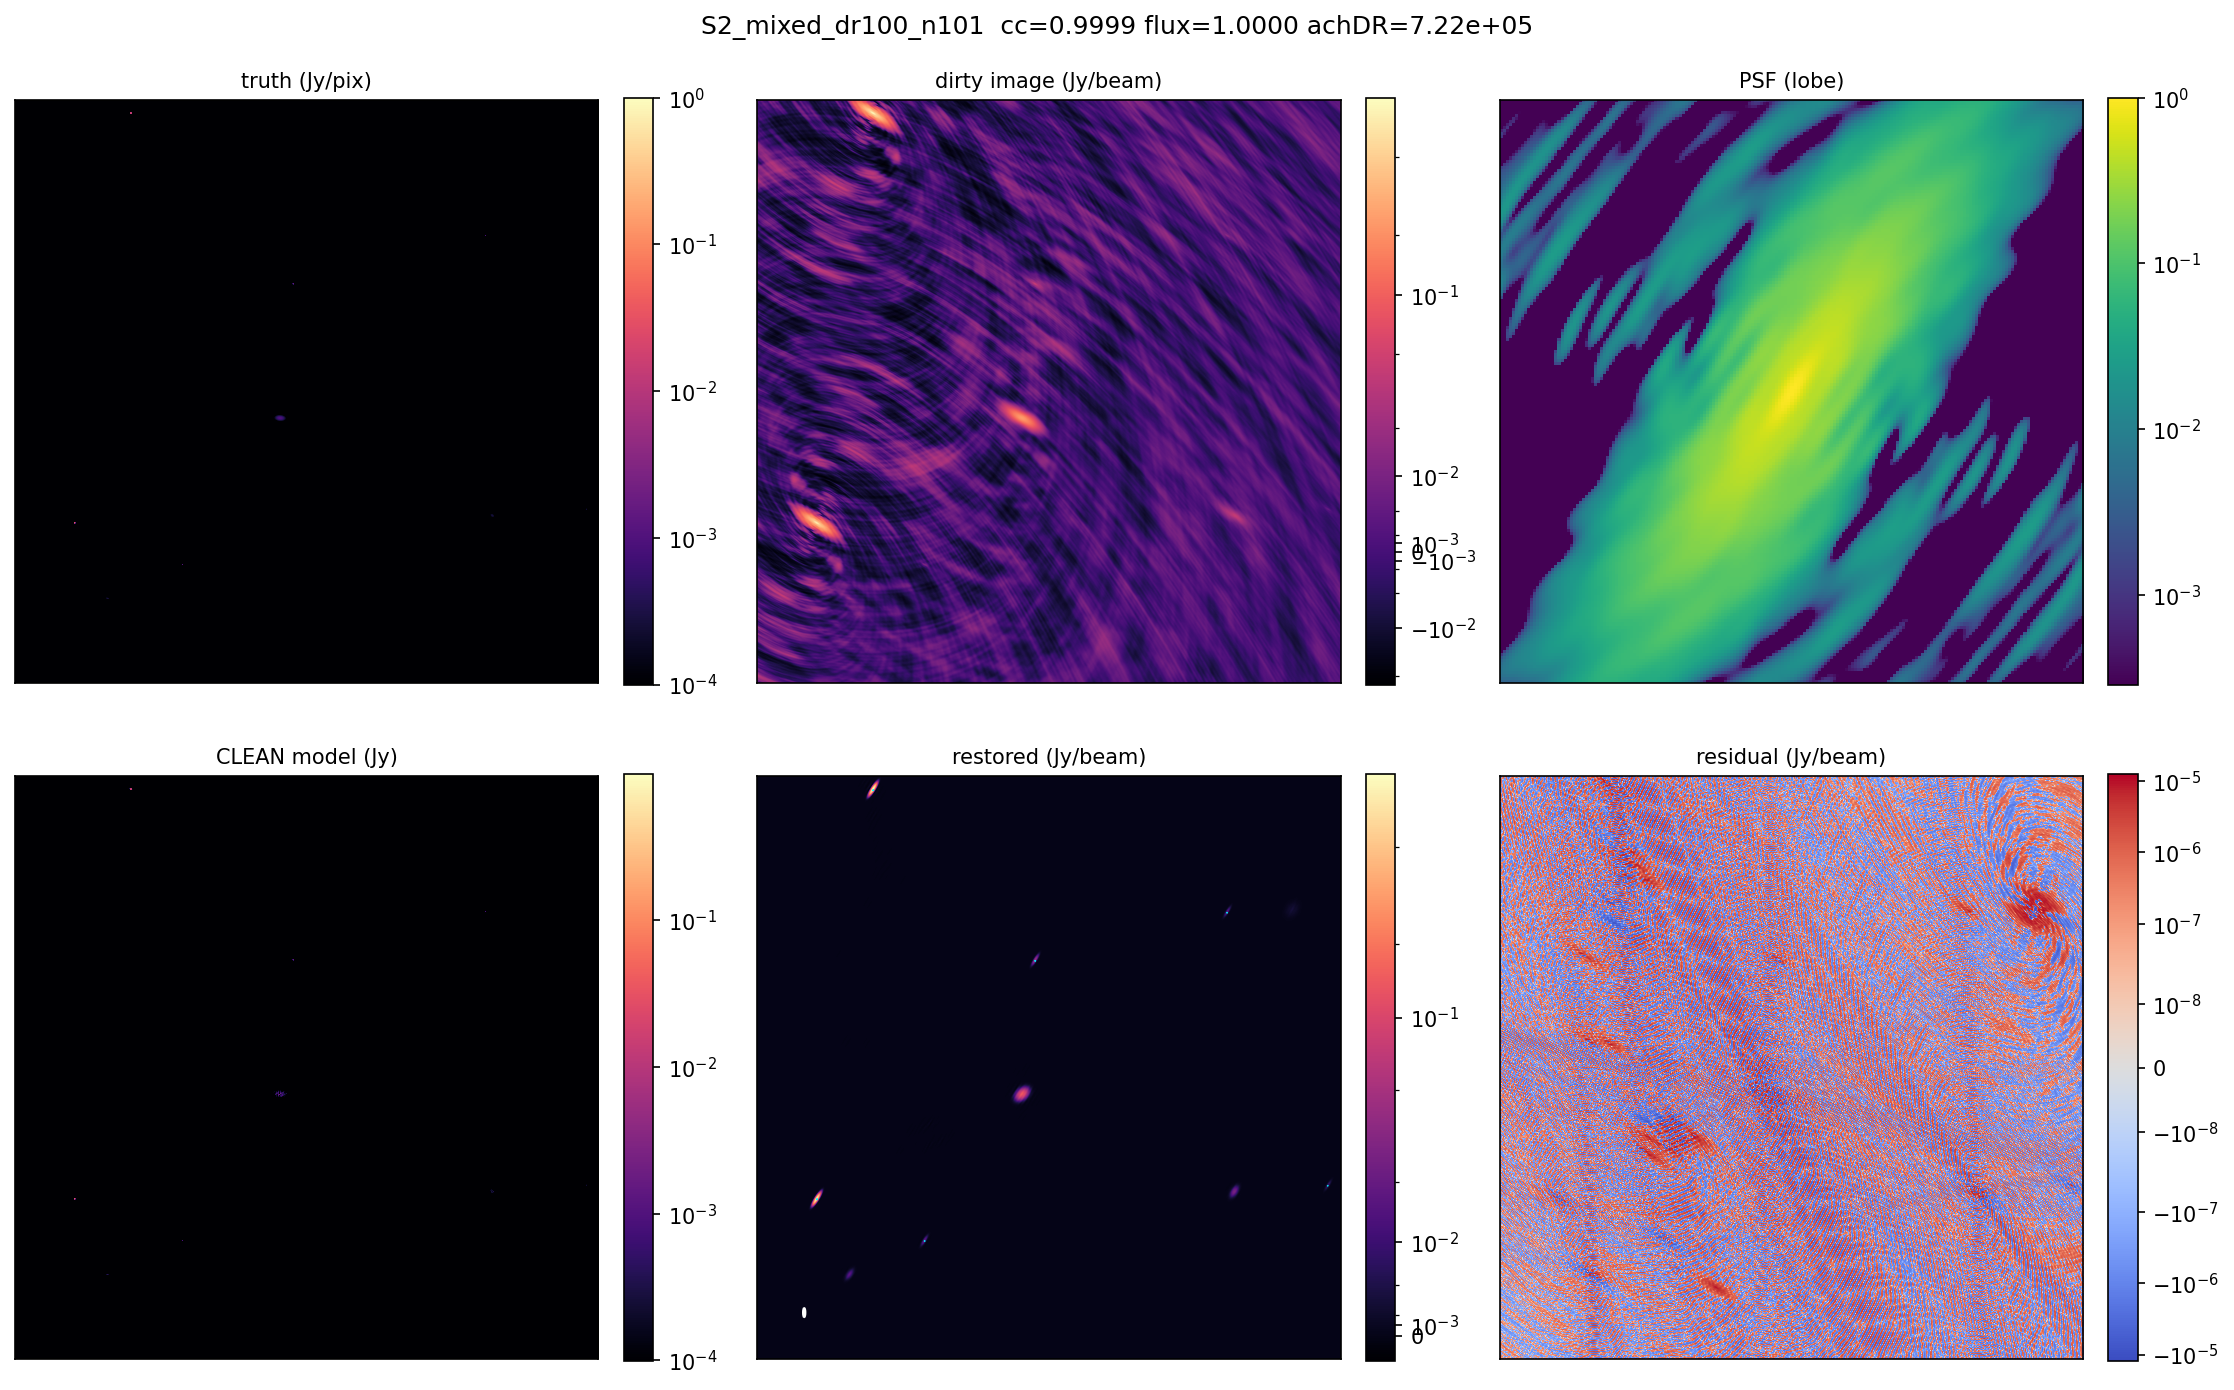
\includegraphics[width=\textwidth]{../analysis/figures/panel_S2_mixed_dr100_n101.png}
\end{frame}

\begin{frame}{Baseline: S3 (gaussians, DR 1000) — images}
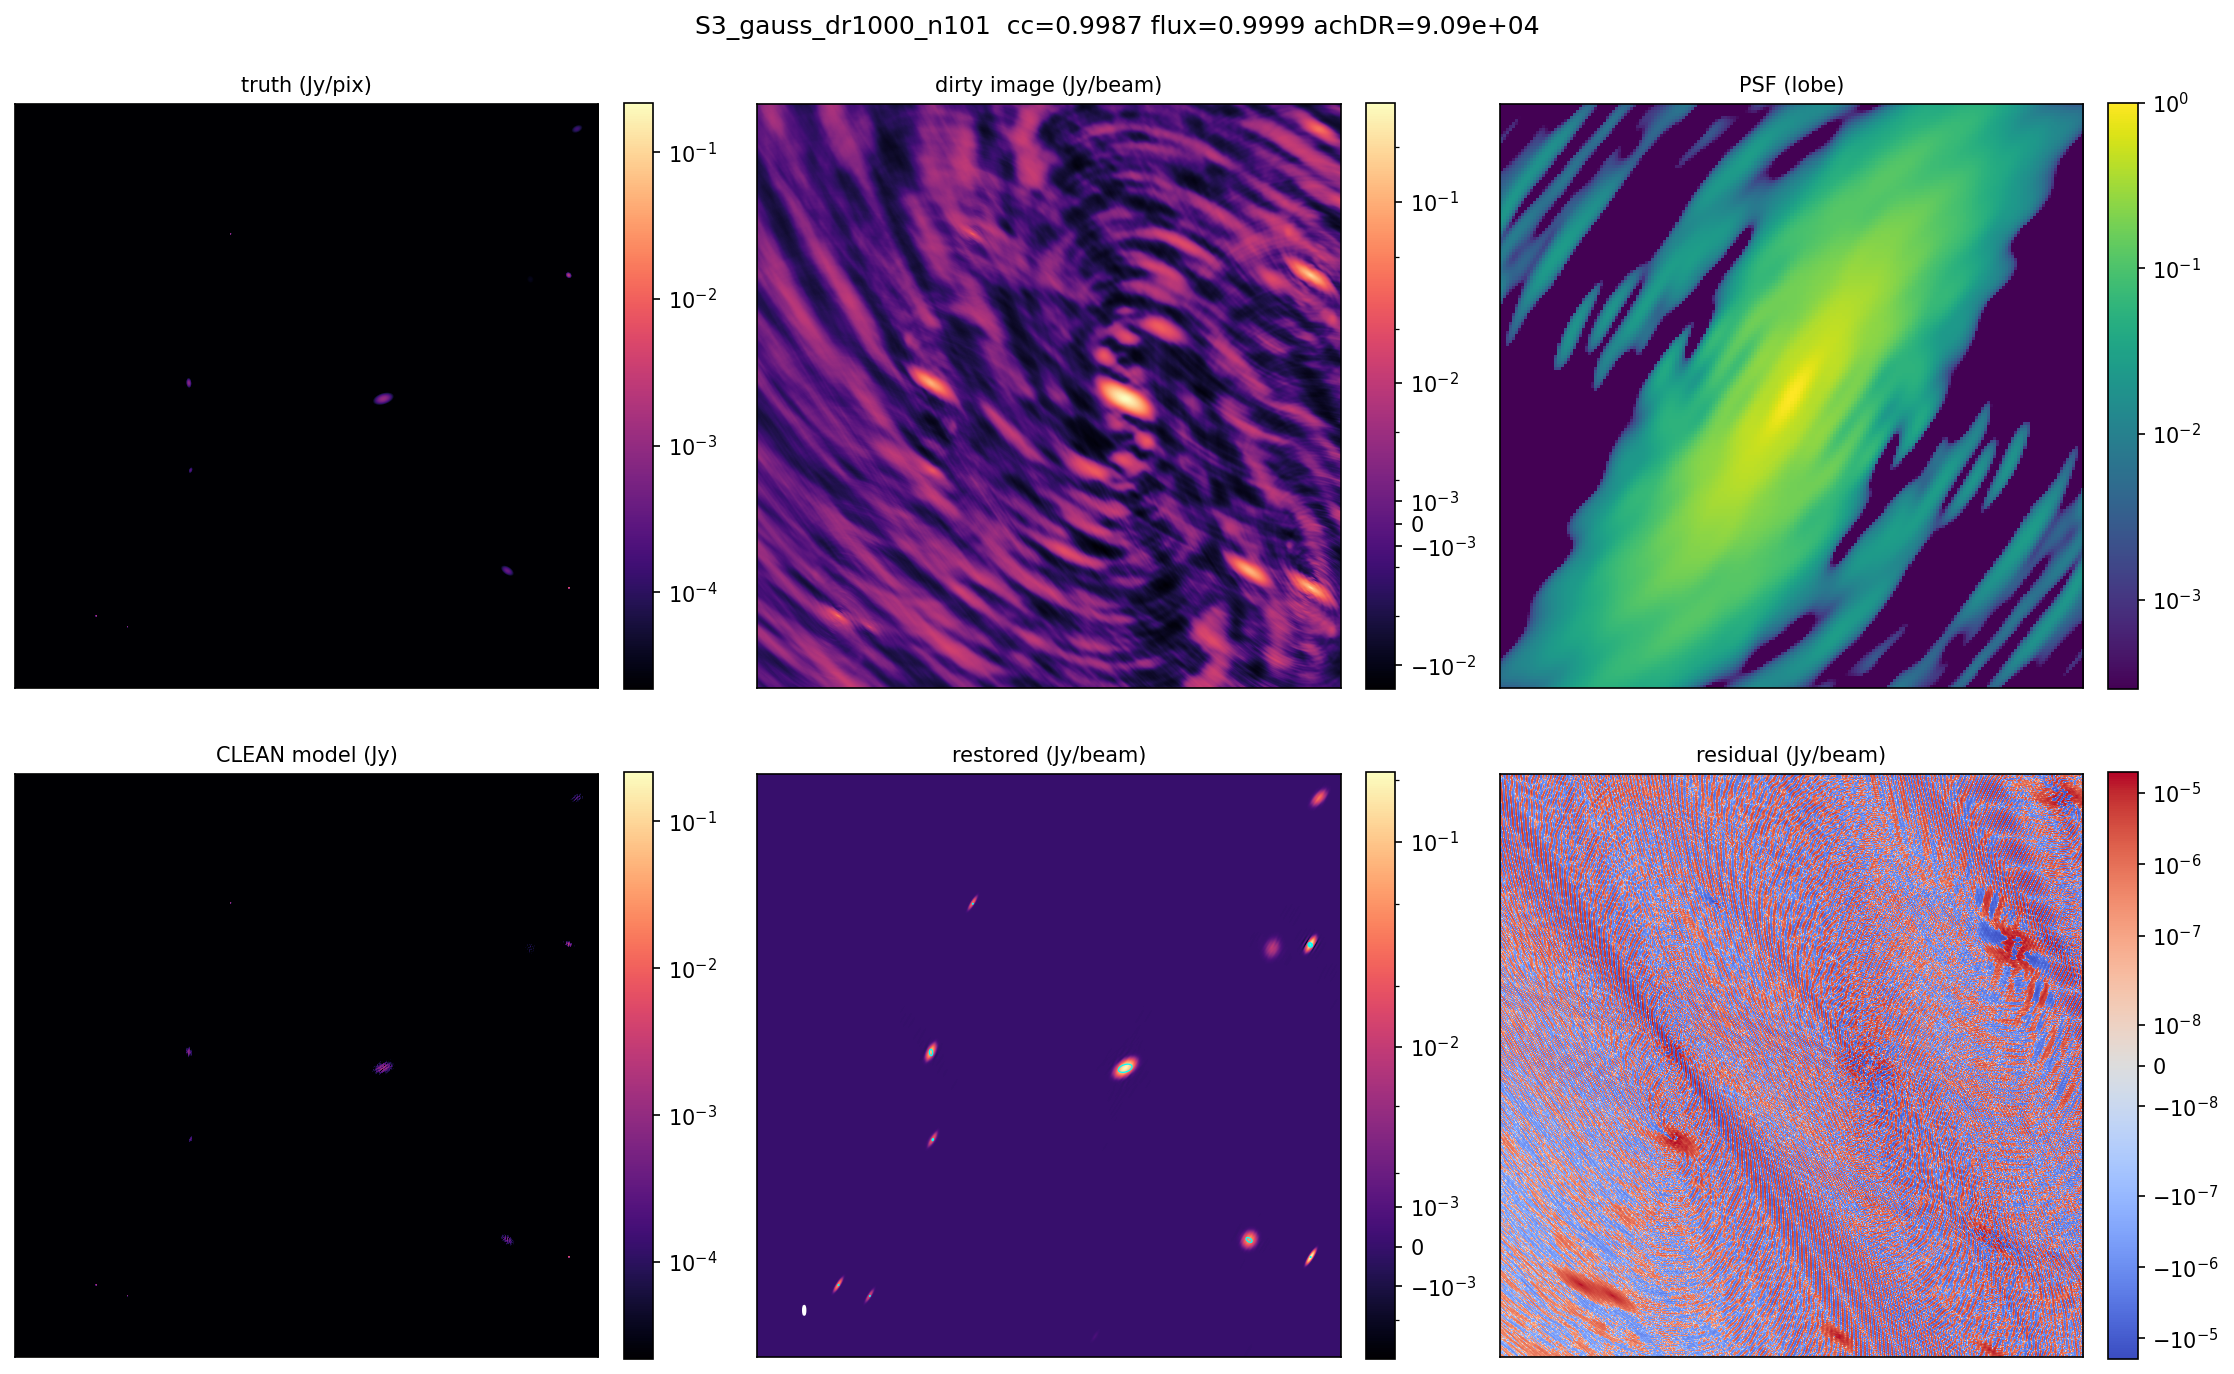
\includegraphics[width=\textwidth]{../analysis/figures/panel_S3_gauss_dr1000_n101.png}
\end{frame}

\begin{frame}{Baseline across the ladder}
\begin{columns}
\begin{column}{0.5\textwidth}
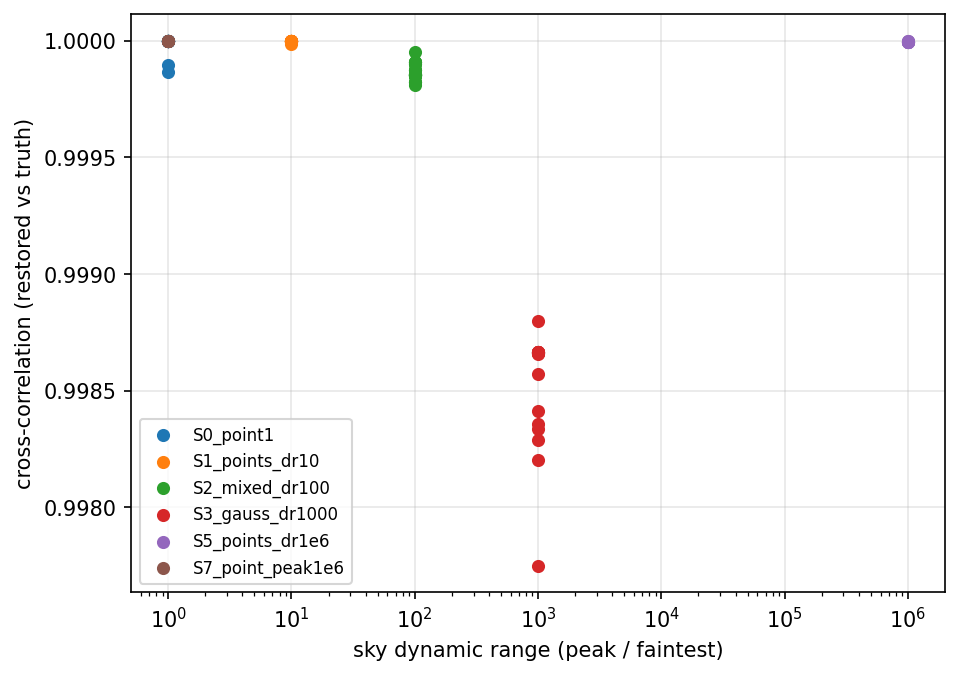
\includegraphics[width=\textwidth]{../analysis/figures/ladder_cc.png}
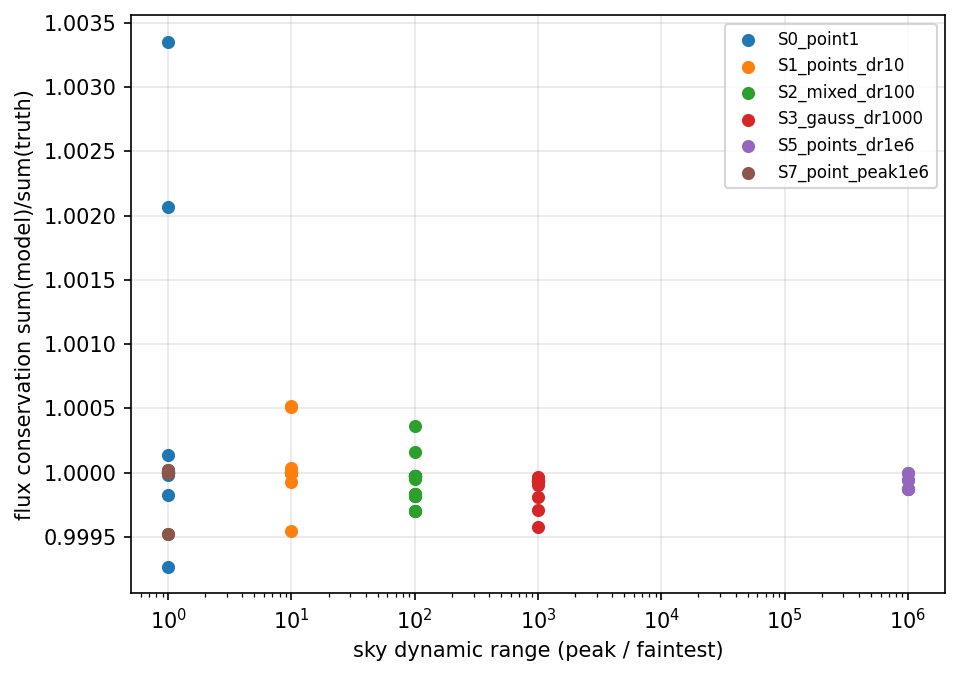
\includegraphics[width=\textwidth]{../analysis/figures/ladder_flux.png}
\end{column}
\begin{column}{0.5\textwidth}
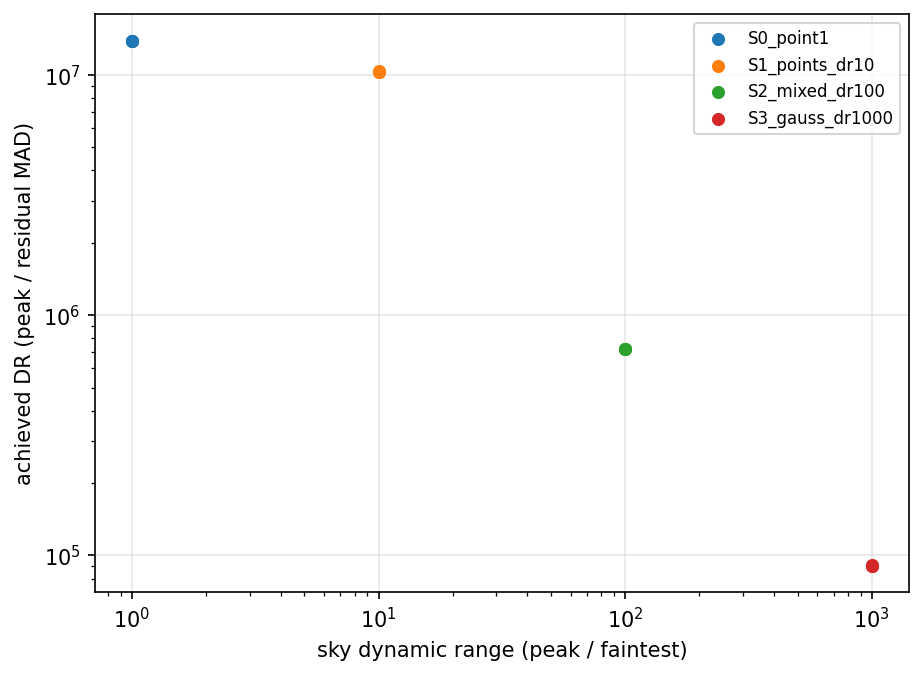
\includegraphics[width=\textwidth]{../analysis/figures/ladder_achdr.png}
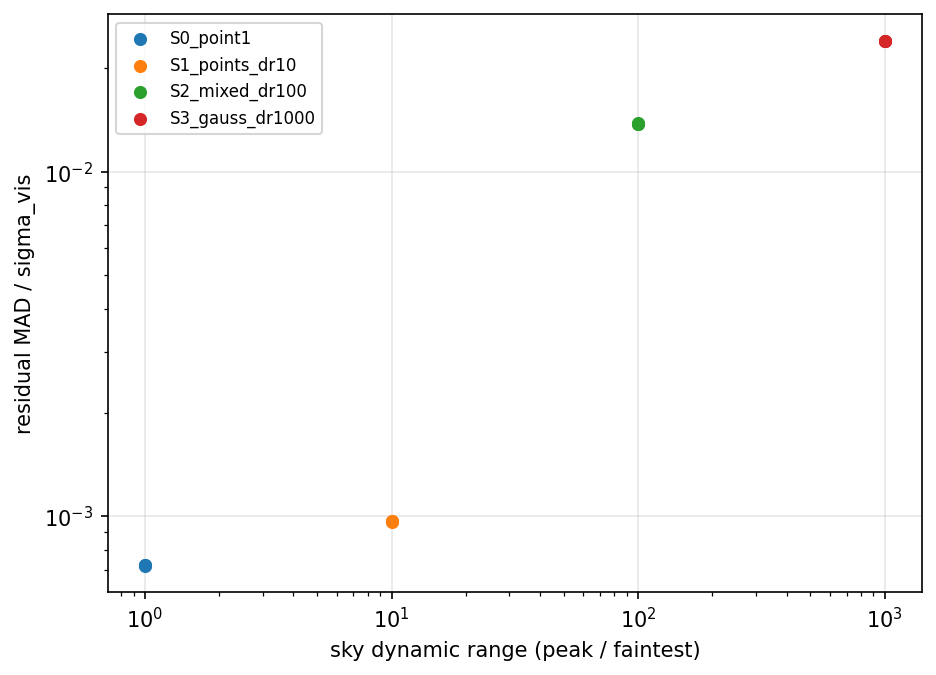
\includegraphics[width=\textwidth]{../analysis/figures/ladder_resmad.png}
\end{column}
\end{columns}
\end{frame}

\begin{frame}{Baseline summary table}
\begin{tabular}{lrrrrr}
\toprule
dataset & seed & cc & flux & res. MAD & ach. DR \\
\midrule
S0\_point1\_n101 & 101 & 1.00000 & 1.00000 & 7.20e-08 & 1.39e+07 \\
S0\_point1\_n101 & 101 & 1.00000 & 1.00000 & 7.20e-08 & 1.39e+07 \\
S0\_point1\_n102 & 102 & 1.00000 & 1.00000 & 7.23e-08 & 1.38e+07 \\
S0\_point1\_n103 & 103 & 1.00000 & 1.00000 & 7.21e-08 & 1.39e+07 \\
S1\_points\_dr10\_n101 & 101 & 1.00000 & 1.00000 & 9.63e-08 & 1.04e+07 \\
S1\_points\_dr10\_n101 & 101 & 1.00000 & 1.00000 & 9.63e-08 & 1.04e+07 \\
S1\_points\_dr10\_n102 & 102 & 1.00000 & 1.00000 & 9.69e-08 & 1.03e+07 \\
S1\_points\_dr10\_n103 & 103 & 1.00000 & 1.00000 & 9.69e-08 & 1.03e+07 \\
S2\_mixed\_dr100\_n101 & 101 & 0.99985 & 0.99997 & 1.38e-06 & 7.22e+05 \\
S2\_mixed\_dr100\_n101 & 101 & 0.99985 & 0.99997 & 1.38e-06 & 7.22e+05 \\
S2\_mixed\_dr100\_n101 & 101 & 0.99985 & 0.99997 & 1.38e-06 & 7.22e+05 \\
S2\_mixed\_dr100\_n101 & 101 & 0.99985 & 0.99997 & 1.38e-06 & 7.22e+05 \\
S2\_mixed\_dr100\_n102 & 102 & 0.99986 & 0.99997 & 1.38e-06 & 7.21e+05 \\
S2\_mixed\_dr100\_n103 & 103 & 0.99986 & 0.99997 & 1.38e-06 & 7.23e+05 \\
S3\_gauss\_dr1000\_n101 & 101 & 0.99866 & 0.99993 & 2.39e-06 & 9.09e+04 \\
S3\_gauss\_dr1000\_n101 & 101 & 0.99866 & 0.99993 & 2.39e-06 & 9.09e+04 \\
S3\_gauss\_dr1000\_n102 & 102 & 0.99866 & 0.99993 & 2.40e-06 & 9.07e+04 \\
S3\_gauss\_dr1000\_n103 & 103 & 0.99866 & 0.99993 & 2.40e-06 & 9.08e+04 \\
S5\_points\_dr1e6\_n101 & 101 & 1.00000 & 1.00000 & 1.14e-07 & 8.73e+06 \\
S5\_points\_dr1e6\_n101 & 101 & 1.00000 & 1.00000 & 1.14e-07 & 8.73e+06 \\
S7\_point\_peak1e6\_n101 & 101 & 1.00000 & 1.00000 & 3.80e-08 & 2.63e+13 \\
S7\_point\_peak1e6\_n101 & 101 & 1.00000 & 1.00000 & 3.80e-08 & 2.63e+13 \\
b2\_S8mix1000\_dr1e4\_s42\_n101 & 101 & 0.99627 & 0.83103 & 6.46e-03 & 148 \\
b2\_S8mix1000\_dr1e4\_s42\_n103 & 103 & 0.99631 & 0.83241 & 6.46e-03 & 148 \\
b2\_S8mix1000\_dr1e4\_s42\_sig1e-2\_n101 & 101 & 0.99627 & 0.83127 & 6.45e-03 & 148 \\
b2\_S8mix1000\_dr1e4\_s42\_sig1e-2\_n102 & 102 & 0.99629 & 0.83111 & 6.46e-03 & 148 \\
b2\_S8mix1000\_dr1e4\_s42\_sig1e-3\_n101 & 101 & 0.99628 & 0.83119 & 6.46e-03 & 148 \\
b2\_S8mix1000\_dr1e4\_s42\_sig1e-3\_n102 & 102 & 0.99627 & 0.83108 & 6.46e-03 & 148 \\
b2\_S8mix1000\_dr1e4\_s42\_sig1e-6\_n101 & 101 & 0.99622 & 0.82931 & 6.53e-03 & 146 \\
b2\_S8mix1000\_dr1e4\_s42\_sig1e-6\_n102 & 102 & 0.99622 & 0.82931 & 6.53e-03 & 146 \\
b2\_S8mix1000\_dr1e4\_s43\_n103 & 103 & 0.99671 & 0.85519 & 5.09e-03 & 259 \\
b2\_S8mix1000\_dr1e4\_s44\_n103 & 103 & 0.99696 & 0.88641 & 3.65e-03 & 260 \\
\bottomrule
\end{tabular}
\end{frame}

\begin{frame}{What the f64 baseline permits us to claim}
\begin{itemize}
\item On point-source fields (S0, S1): CLEAN is essentially exact
  (cc $=1$, flux $=1$, residual at the noise floor $\sigma/\sqrt{N}$) —
  quantization effects here are pure numerics, measurable cleanly.
\item On Gaussian fields (S2, S3): delta-Högbom leaves an extended-emission
  residual above the noise floor — this bounds any claim about extended
  sources, and is where quantization of the model/PSF will matter most.
\item Achieved DR is noise-limited, not pf-limited: $pf=10^{-4}$ stops far
  above the noise floor, so DR is set by $\sigma$.
\item Next: the 16 quantization schemes on this same ladder, compared to these
  f64 references within the 3-seed spread.
\end{itemize}
\end{frame}

\end{document}
